\chapter{根与翼} % Introduction chapter suppressed from the table of contents


团队和企业要健康成长依赖以下主要因素(与上一章创新的要素类似):\\

\begin{itemize}
\item
  高层要制订高的目标,也要提供资源。

  \begin{itemize}
  \tightlist
  \item
    可参考开始过程改进之旅里面的获取高层支持,尽早估算改进能节省多少成本,要求立项,把过程改进作为项目来管理。
  \end{itemize}
\item
  改进要有专注。

  \begin{itemize}
  \tightlist
  \item
    例如针对如何减少缺陷返工,尽早在评审和前期测试发现缺陷,如何做好迭代回顾部分能帮助团队了解应如何开始。
  \end{itemize}


\item
  团队成员的能力与动力。

  \begin{itemize}
  \tightlist
  \item
    个人提升、自我管理、代码质量等部分能帮助提升。
  \end{itemize}
\end{itemize}

有竞争才有进步,不知道自身的不足,缺乏危机感是改善的最大阻力。

\framebox{%
\begin{minipage}[t]{0.97\columnwidth}\raggedright
东北虎作为濒危物种,目前在国内的数量估计不超过30只,因此国家动物保护组织采取了多项措施予以保护,其中包括人工饲养。专家曾试图将这些人工饲养的东北虎重新放归野外,但这一任务极为艰巨。它们是否能够在野外独立存活下来,仍然是一个未知数。有一部纪录片生动地讲述了动物保护组织在这一过程中所面临的各种挑战和困难。\\
我们经过严格的筛选,挑选出最具潜力的老虎。第一次选中的是一只年轻且体型较大的老虎,将其放到一个模拟自然环境的大型操场,供专家进行观察。刚开始,这只老虎还是表现出了典型野生老虎的特征,如:警惕地观察周围的环境等。然而,几小时后,这只老虎没有抵抗住低温环境,还是选择回到自己的巢穴,这次尝试失败了。另一只被选中的老虎虽然充满活力,也不怕冷,但却缺乏野生动物的警惕性,它已经习惯了人类的存在,这可能会给它的野外生活带来危险。因此,专家不得不放弃了这只老虎。\\
要确保老虎在野外能独立生存,它们必须能够自行觅食。在自然环境中,它们主要的捕猎对象就是鹿,但鹿非常敏捷,时速可达五十公里,而且具备很强的耐力。因此,专家需要评估老虎是否能够成功捕猎到鹿,否则就不能将它们放归到野外。在评估过程中,专家发现老虎的奔跑和狩猎能力明显不如野生老虎,因为缺少运动,它们缺乏狩猎的能力。因此,专家设计了多种锻炼方法,如使用车辆牵引轮胎,并插上鲜肉块来刺激它们奔跑。经过一系列的锻炼,老虎的体力得到了恢复,但能否成功捕猎到鹿仍然是未知数。\\
另一个试验是用汽车拖着鹿的尸体,以此吸引老虎奔跑。然而,有些老虎因为在平时的饲养过程中并没有吃过鹿肉,所以对此并不感兴趣。最终,只有两三只老虎追着汽车跑,试图抓到鹿。最后,有两只年轻的老虎获胜了。但要将鹿的尸体作为奖励喂给获胜的老虎也并不容易,发现它们对着鹿的尸体不知道如何下口,因为以前都是由饲养员将肉切好后喂给它们吃。最终,这两只老虎花了数小时才慢慢学会如何吃到鹿肉。

\strut
\end{minipage}}

环境是影响团队能力与动力的重要因素。看完这部纪录片,我立刻想到了有些年轻的程序员,他们也是在相对受到保护的环境下工作。这些程序员可能已习惯了管理层或经验丰富的同事对他们的代码质量要求并不高。因此,如果我们希望这些年轻的程序员注重代码质量,就跟保护区把饲养的东北虎放归野外一样,需要经过艰苦的培训,以提高他们的竞争力。管理层必须认识到,只是一味地保护程序员,对他们提供高质量的代码没有要求,那么公司的产品质量将永远无法提高,也难以与其他公司竞争。\\
中国社会一直非常强调家庭价值观,希望实现家族的持续传承,家族有族谱,代代相传的关系对每个家庭成员的成长产生深远影响。我们每个人都只是人类进化过程中的短暂过渡。父母普遍希望把最好的东西传承给下一代。然而,我们需要问自己,什么东西能够持久,仅仅是财富和金钱吗?\\
继承大量财富,但如果不懂得如何正确利用,可能反而会削弱个人的竞争力,适得其反,最终成为社会的蛀虫。\\
《七个习惯》的作者史蒂芬•柯维(Stephen
Covey)在书的结尾(最后一章)中提到,我们可以传承给下一代并具有持久价值的,只有两样东西:根和翼。\\
`There are only two lasting bequests we can give our children - one is
roots, the other wings.'

\hypertarget{ux6839}{%
\subsection{根}\label{ux6839}}

回看人类过去130年,除了打了两次世界大战外,也做了很多前所未有的创新:

\begin{itemize}
\tightlist
\item
  电灯 (煤气灯)
\item
  汽车 (马车)
\item
  飞机
\item
  摩天大厦
\item
  半导体,集成电路
\item
  计算机
\item
  互联网
\item
  移动电话
\end{itemize}

人类创新并不仅限于前述领域,这只是我们看到的凤毛麟角,其他在医疗、电影、音乐、数学等各个领域都表现出了卓越的创新力,这些都是祖先留给我们的宝贵财富。\\
举例来说,如果十九世纪欧洲城市的居民能够坐上像"Back to the
Future"那样的时间跑车,见到两百年后现代人的生活,他们将感到难以置信。\\
然而,当我们观察现代社会的儿童和年轻人时,由于不再需要担心衣食住行,他们往往将更多的精力投入到虚拟世界的游戏、养宠物、以及在线购物等方面,这确实引发了一些担忧。\\
有人可能会提出反对意见,说:``我不是贝多芬,也不是乔布斯,我没有像他们那样非凡的魄力。''

\hypertarget{ux7ffc}{%
\subsection{翼}\label{ux7ffc}}

除了根的传承,祖先还留给了我们``翅膀'',赋予了我们自由的能力,以此打破负基因的传承,追求改善、变革和创新,而不是简单地将这些基因传给下一代。\\
To be a powerful transition person, one must first change his inner
first.\\
我们每个人都只是在人类几万年进化历程中的一个瞬间。必须先从内而外做改变,才可以持久。要成为一位有影响力的过渡者,我们必须首先进行由内而外的改变,这样的改变才能持久。\\
当然,我们也可以在自己可控的范围内进行创新和持续改善。\\

从下面故事能看到成功非偶然,都必须经过不断从失败中改进的过程。

\hypertarget{ux98deux884cux5b9eux9a8c}{%
\subsubsection{飞行实验}\label{ux98deux884cux5b9eux9a8c}}

人类一直都想飞上天,中西方对此都有尝试。例如,传说明代火箭专家万户陶成道尝试在凳子上绑47根火箭,又绑上风筝做飞行试验,结果爆炸而亡。15世纪,意大利人达芬奇也模仿鸟类的翅膀设计飞行器,但只是留在图纸设计阶段。

\framebox{%
\begin{minipage}[t]{0.97\columnwidth}\raggedright
韦德兄弟 (Wright brothers) 1903年首次机动飞机飞行成功\\
莱特兄弟1903年首次成功飞行,在12月17日的第四次飞行在空中飞行了59秒,航程达到259米。

%\href{文件:1903wrightScreenshot_2022-02-14_103500.jpg}{300px}\\
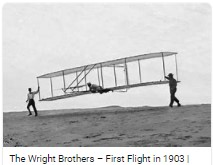
\includegraphics[width=10cm]{1903wrightScreenshot_2022-02-14_103500.jpg}

莱特兄弟并非工程或数学天才(他们都没有读过大学),但为了实现``飞翔''的梦想,不断从失败找改进,从1899年开始不断试验:\\
1900年,他们首次试验滑翔机,但效果并不理想。\\
1901年,他们把机翼的面积从15扩大到26平米,可以飞行120米,但他们发现试验数据与计算数据不符。为了找出原因,他们制造了风洞来测量各种机翼设计的浮力。他们试验了200种机翼。利用收集数据,他们开始制作第三架滑翔机。\\
1902年9月份,他们完成了1000次试飞,其中空中飞行最长可以达到26秒。也因为这些经验,他们知道如何设计飞机的舵,让飞行员更好控制飞机,并开始设计使用4气缸发动机加上螺旋桨(设计原理和机翼设计相同)准备设计机动飞机。\\
1903年成功飞行后,他们继续改善设计。1905年10月,飞机能在空中飞行39分钟,并且能在飞行员控制下转圈。\\
飞行是在不稳定的大气条件下操控不稳定的机器,充满了许多变数,因此非常困难。最终,韦德兄弟通过不断实验,自己发明了飞机各种重要部件,包括机翼、舵、发动机、螺旋桨等,并研究了它们之间是如何相互影响。
\strut
\end{minipage}}

从莱特兄弟的飞行故事,可以看到创新不是单靠创新的意念,更重要是不断试验,从失败中获取经验教训,收集数据持续改进。\\
1985年乔布斯被迫离开苹果公司,独资开创
NEXT公司,到1997年NEXT被苹果公司收购,乔布斯重返苹果(当时苹果公司在破产边缘),到2010年将苹果公司带回到美国市值最高的科技公司,中间也经历了多次失败。\\
丰田公司从二战后快破产到后来成为世界第一,也非一帆风顺。\\

\hypertarget{tedux6f14ux8bb2ux5f0fux603bux7ed3}{%
\subsection{TED演讲式总结}\label{tedux6f14ux8bb2ux5f0fux603bux7ed3}}

今年被质量经理邀请参加他们的质量沙龙,但只有30分钟,我就用了TED演讲思路,用了17分钟讲软件开发公司的常见质量问题和改进措施。

\framebox{%
\begin{minipage}[t]{0.97\columnwidth}\raggedright
你觉得下面4种工作,哪一类工种占的工作量最多?

\begin{enumerate}
\tightlist
\item
  编码与代码设计。
\item
  交付后的所有工作,包括维护、更新与缺陷修正。
\item
  交付前的评审、静态扫描、测试与缺陷修正。
\item
  项目管理与监控。
\end{enumerate}

从Capers Jones
2012年对美国软件公司的统计,编码只是排第二(占开发工作量的25\%),测试与评审和缺陷修改的总工作量才是排第一(占30\%)。你选1.编码,其实大部分耗时的不是写代码,而是修正错误代码。软件开发有特点,缺陷发现越晚,修改耗费的工作量就越大。如果早期发现,可能只需要花费半小时、1小时修正。原因很简单,当已经集成为一个十几万行的系统,里面有很多组件。如果集成完成后使用时才发现BUG,首先很难找出是哪里代码出问题,然后为了验证代码修正对不对,首先要测试单元模块通不通过,再测集成通不通,最后也通过系统测试才能给客户。但是如果前面自己自测、集成测试、评审时尽早发现并解决问题,便能节省了很多时间。\\
但是公司大部分的缺陷都是在系统测试或集成测试时暴露,有些产品线的缺陷数甚至达到4位数。如果可以把这些缺陷减少一半,能为公司节省下接近一半工作量,同时也改善产品质量,对吗?\\
这道理大家都知道,但是为什么没有改善?怎样才能改变现状,提前发现缺陷?\\
这种改进绝对不能下达一个命令,或者领导开会讲讲就能做到。我先说一个故事,有一家上万人的大型公司,质量经理说公司一直都非常注重量化管理,定了各种KPI给团队遵守,每个月主管分析数据。发现开始时是有些改善,但过了一段时候,后面作用就不大了。而且当那些数字变成KPI以后,发现有数字作假。所以我跟做分析的质量经理说,如果希望量化管理就必须要从团队提升开始,而不是靠总体数据分析,制订公司级改进策略。度量与分析最主要的作用是帮助团队做好根因分析,制订纠正措施,在下一轮迭代做提升。\\
比如你们现在都是按2~4周一次发版迭代,有些团队确实也有做复盘,但是他们不理解纠正措施和改正的区分,他们只是针对个别的缺陷去修改,这种还是会导致因为没有修正系统的基本问题,缺陷、事故还是会重现。但是如果我们整个团队每轮迭代分析数据,找根因,制订纠正措施,在下一个迭代验证是否有效。要养成这个习惯,最重要还是要团队动起来。首先领导要给他们有充足的时间去做复盘。要做好这种根因分析的复盘差不多要三个小时,因为要收集数据、分析和讨论。\\
我们可以先从分析缺陷排除率开始,让团队开始养成复盘分析根因的习惯。缺陷有真实数据,让团队分析为什么需求引入的缺陷这么多?引导团队一起用``五个为什么''找出根因。让团队人员知道现在的质量水平。一般问需求人员自己质量水平怎么样?他很会说我们需求评审发现很少BUG,代表质量好。其实他误解了一些结果成绩的度量和过程的度量。他在评审过程里面没有发现不表示需求没缺陷,等到客户发现缺陷更糟糕。\\
我们也可以利用一些预测模型、统计分析的方法。在迭代里让团队不仅制订纠正措施,也有定量化目标,例如需求评审应该发现多少缺陷?单元测试应该发现多少缺陷?如果没达到预计范围,表示很可能还是有不少缺陷会遗漏到后面。所以按这个目标就可以更好驱动他做好前面的评审和单元测试。
如果团队开始有分析根因并制订纠正措施的习惯,领导也一直关注团队的持续改进,会不时问:“下次迭代?改进了多少?”,就可以把根因分析扩大。除了分析缺陷外,也可以扩大根因分析其他改进方向。\\
怎么可以开始?\\
只是把小孩扔进海里,他是学不会游泳的。所以通常建议先进行培训,举办两天的工作坊,用一些实际的数据,带领大家做一些互动根因分析练习,然后再公司内部教练辅导团队,帮助他们做好迭代里复盘。\\
\strut
\end{minipage}}

与企业领导的首次见面,我也会讲以上内容,说明团队可以如何分析迭代缺陷数据,开始定量管理。\\
针对软件开发,我们这一代继承了之前从60年代以来的各种硬件软件的创新,给予我们继续发展的``根''。\\
敏捷宣言指出了传统瀑布式开发和传统计划驱动开发的弊端,给我们``翼'',为有能力的团队提供了机会,可以更快速地开发出高质量的产品。\\
千万不要误以为这过程会一帆风顺,按计划执行就能达到目标。实际肯定会遇到种种无法预料的问题,但只要个人、团队、企业了解当前水平,分析根因,采取纠正措施、持续改善,像第一章丰田方式的习惯4:“持续改善没有停止”  --  龟兔赛跑里的乌龟。\\
不怨天忧人,\\
分析投诉和意见,\\
归纳成经验教训,\\
不断改善,\\
你便能每天成长;\\
制订改进目标,\\
定期利用数据复盘,\\
一起分析根因,\\
执行纠正措施,\\
团队便能每月进步。\\
以上简单道理不仅适用于敏捷开发,回顾周围有多少人、团队能做到?\\

\framebox{%
\begin{minipage}[t]{0.97\columnwidth}\raggedright
乔布斯在他的传记里说,“是什么力量推动我? 我觉得大多数具创意者(Creative people) 都很希望感谢我们的前辈,感激他们对人类的贡献。\\
我并没有发明我用的语言或数学。我的食物基本都不是我自己做的,衣服更是一件都没做过。我所做的每一件事都有赖于我们人类的其他成员,以及他们的贡献和成就。我们很多人都想回馈社会,在历史的长河中再添上一笔。我们只能用这种大多数人都掌握的方式去表达——因为我们不会写鲍勃·迪伦的歌或汤姆·斯托帕德(Tom Stoppard)的戏剧。我们试图用我们仅有的天分去表达我们深层的感受,去表达我们对前人所有贡献的感激,去为历史长河加上一点儿什么。那就是推动我的力量。”\\
\strut
\end{minipage}}

反观,我的动力是什么?虽然软件工程发展历史不长(50年代才出现第一台大型计算机),但发展速度惊人,环顾周围,几乎难以找到没有附带软件的产品。 
在此过程中,我们受益于软件工程的前辈,包括软件工程学院的 Humphrey先生,发表敏捷宣言的17位敏捷大师等,以及质量改善和组织发展 (Organization Development))学者的研究,如裘兰博
士 、Lewin 教授、Weibord先生等。希望在我有限的能力和时间内,尽可能系统地总结这二十多年与软件团队交流中的所见所闻和经验教训,解读敏捷开发最佳实践,方便大家参考。也希望各位同仁可以找到驱动个人或团队改善的动力,沿着前辈的步伐一路前行,持续改善。 

\hypertarget{ux53c2ux8003-references}{%
\section{参考 References}\label{ux53c2ux8003-references}}

\begin{enumerate}
\tightlist
\item
  Covey, Stephen R. ''The Seven Habits of Highly Effective People.'' (1990) Fireside Book 
\item
   Isaacson, Walter. ''Steve Jobs.'' (2011)
\end{enumerate}



